\documentclass{standalone}
\usepackage{tikz}
\usetikzlibrary{patterns, positioning}

\begin{document}
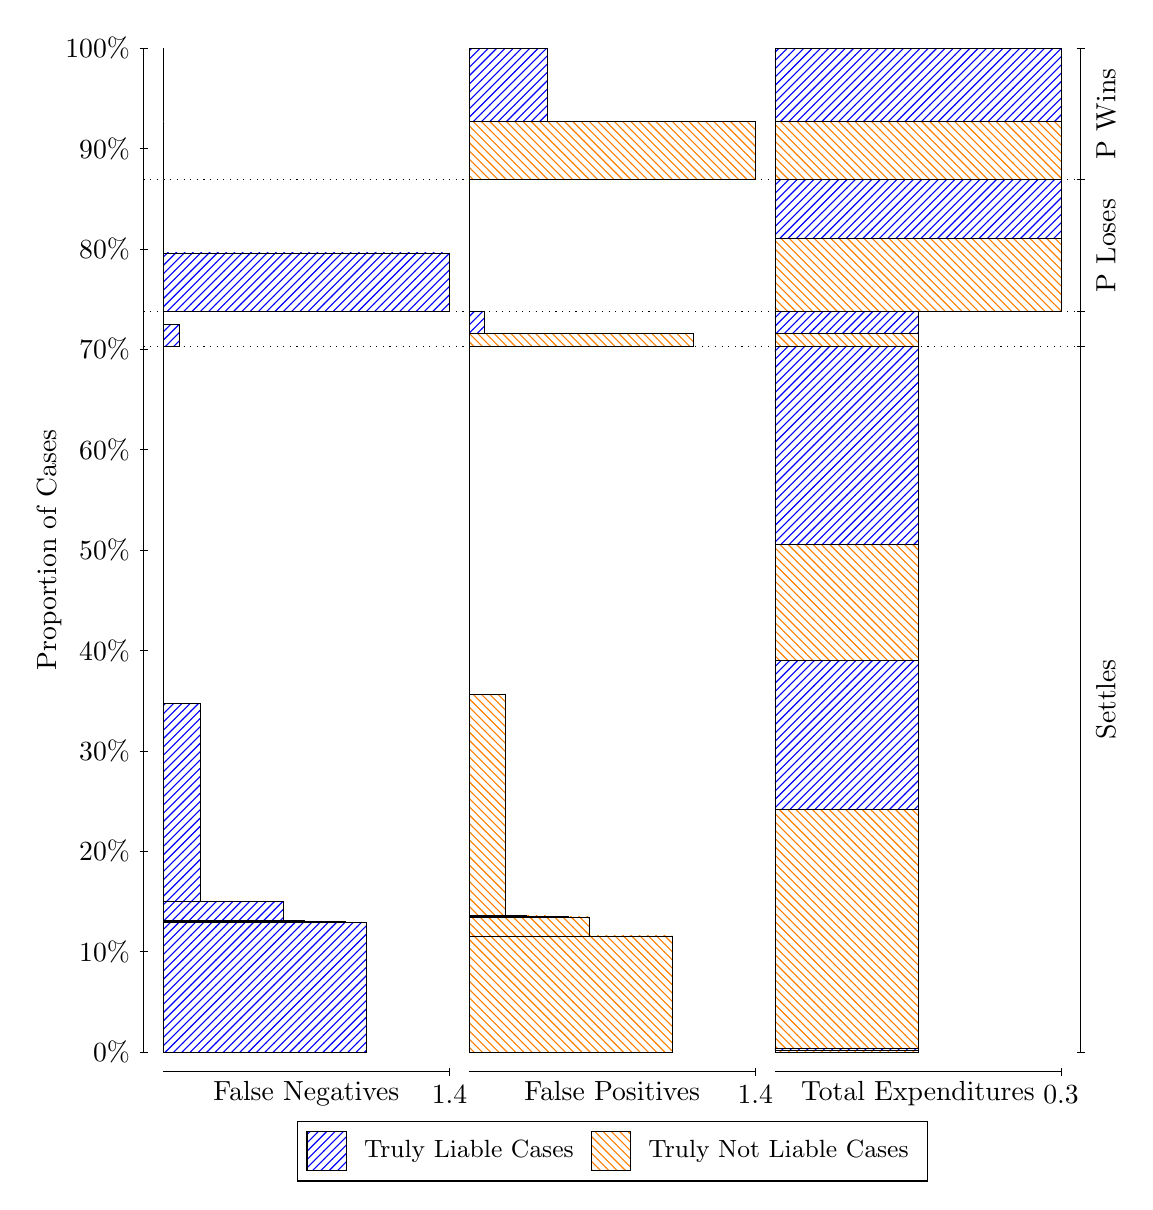
\begin{tikzpicture}
\draw[black, very thin] (1.5,1.75) -- (1.5,14.5);
\node[rotate=90, anchor=center] at (0.3, 8.125) {Proportion of Cases};
\draw[black, very thin] (1.45,1.75) -- (1.55,1.75);
\node[anchor=east] at (1.45, 1.75) {0\%};
\draw[black, very thin] (1.45,3.025) -- (1.55,3.025);
\node[anchor=east] at (1.45, 3.025) {10\%};
\draw[black, very thin] (1.45,4.3) -- (1.55,4.3);
\node[anchor=east] at (1.45, 4.3) {20\%};
\draw[black, very thin] (1.45,5.575) -- (1.55,5.575);
\node[anchor=east] at (1.45, 5.575) {30\%};
\draw[black, very thin] (1.45,6.85) -- (1.55,6.85);
\node[anchor=east] at (1.45, 6.85) {40\%};
\draw[black, very thin] (1.45,8.125) -- (1.55,8.125);
\node[anchor=east] at (1.45, 8.125) {50\%};
\draw[black, very thin] (1.45,9.4) -- (1.55,9.4);
\node[anchor=east] at (1.45, 9.4) {60\%};
\draw[black, very thin] (1.45,10.675) -- (1.55,10.675);
\node[anchor=east] at (1.45, 10.675) {70\%};
\draw[black, very thin] (1.45,11.95) -- (1.55,11.95);
\node[anchor=east] at (1.45, 11.95) {80\%};
\draw[black, very thin] (1.45,13.225) -- (1.55,13.225);
\node[anchor=east] at (1.45, 13.225) {90\%};
\draw[black, very thin] (1.45,14.5) -- (1.55,14.5);
\node[anchor=east] at (1.45, 14.5) {100\%};

\draw[black, very thin] (13.4,1.75) -- (13.4,14.5);
\draw[black, very thin] (13.35,1.75) -- (13.45,1.75);
\node[anchor=west] at (13.35, 1.75) {};
\draw[black, very thin] (13.35,10.709) -- (13.45,10.709);
\node[anchor=west] at (13.35, 10.709) {};
\draw[black, very thin] (13.35,11.156) -- (13.45,11.156);
\node[anchor=west] at (13.35, 11.156) {};
\draw[black, very thin] (13.35,12.828) -- (13.45,12.828);
\node[anchor=west] at (13.35, 12.828) {};
\draw[black, very thin] (13.35,14.5) -- (13.45,14.5);
\node[anchor=west] at (13.35, 14.5) {};

\draw[black, very thin, pattern color=blue, pattern=north east lines] (1.75,1.75) rectangle (4.3264,3.398);
\draw[black, very thin, pattern color=blue, pattern=north east lines] (1.75,3.398) rectangle (4.0621,3.4049);
\draw[black, very thin, pattern color=blue, pattern=north east lines] (1.75,3.4049) rectangle (3.7979,3.4121);
\draw[black, very thin, pattern color=blue, pattern=north east lines] (1.75,3.4121) rectangle (3.5336,3.4193);
\draw[black, very thin, pattern color=blue, pattern=north east lines] (1.75,3.4193) rectangle (3.2694,3.6597);
\draw[black, very thin, pattern color=blue, pattern=north east lines] (1.75,3.6597) rectangle (2.2124,6.1724);
\draw[black, very thin, pattern color=orange, pattern=north west lines] (1.75,6.1724) rectangle (1.75,10.709);
\draw[black, very thin, pattern color=blue, pattern=north east lines] (1.75,10.709) rectangle (1.9482,10.99);
\draw[black, very thin, pattern color=orange, pattern=north west lines] (1.75,10.99) rectangle (1.75,11.156);
\draw[black, very thin, pattern color=blue, pattern=north east lines] (1.75,11.156) rectangle (5.3833,11.898);
\draw[black, very thin, pattern color=orange, pattern=north west lines] (1.75,11.898) rectangle (1.75,12.828);
\draw[black, very thin, pattern color=orange, pattern=north west lines] (1.75,12.828) rectangle (1.75,13.569);
\draw[black, very thin, pattern color=blue, pattern=north east lines] (1.75,13.569) rectangle (1.75,14.5);
\draw[black, very thin, pattern color=orange, pattern=north west lines] (5.6333,1.75) rectangle (8.2097,3.2247);
\draw[black, very thin, pattern color=orange, pattern=north west lines] (5.6333,3.2247) rectangle (7.1527,3.4649);
\draw[black, very thin, pattern color=orange, pattern=north west lines] (5.6333,3.4649) rectangle (6.8885,3.4722);
\draw[black, very thin, pattern color=orange, pattern=north west lines] (5.6333,3.4722) rectangle (6.6242,3.4794);
\draw[black, very thin, pattern color=orange, pattern=north west lines] (5.6333,3.4794) rectangle (6.36,3.4864);
\draw[black, very thin, pattern color=orange, pattern=north west lines] (5.6333,3.4864) rectangle (6.0958,6.2869);
\draw[black, very thin, pattern color=blue, pattern=north east lines] (5.6333,6.2869) rectangle (5.6333,10.709);
\draw[black, very thin, pattern color=orange, pattern=north west lines] (5.6333,10.709) rectangle (8.4739,10.876);
\draw[black, very thin, pattern color=blue, pattern=north east lines] (5.6333,10.876) rectangle (5.8315,11.156);
\draw[black, very thin, pattern color=orange, pattern=north west lines] (5.6333,11.156) rectangle (5.6333,12.087);
\draw[black, very thin, pattern color=blue, pattern=north east lines] (5.6333,12.087) rectangle (5.6333,12.828);
\draw[black, very thin, pattern color=orange, pattern=north west lines] (5.6333,12.828) rectangle (9.2667,13.569);
\draw[black, very thin, pattern color=blue, pattern=north east lines] (5.6333,13.569) rectangle (6.6242,14.5);
\draw[black, very thin, pattern color=orange, pattern=north west lines] (9.5167,1.75) rectangle (11.333,1.7715);
\draw[black, very thin, pattern color=blue, pattern=north east lines] (9.5167,1.7715) rectangle (11.333,1.7928);
\draw[black, very thin, pattern color=orange, pattern=north west lines] (9.5167,1.7928) rectangle (11.333,4.8335);
\draw[black, very thin, pattern color=blue, pattern=north east lines] (9.5167,4.8335) rectangle (11.333,6.7219);
\draw[black, very thin, pattern color=orange, pattern=north west lines] (9.5167,6.7219) rectangle (11.333,8.1966);
\draw[black, very thin, pattern color=blue, pattern=north east lines] (9.5167,8.1966) rectangle (11.333,10.709);
\draw[black, very thin, pattern color=orange, pattern=north west lines] (9.5167,10.709) rectangle (11.333,10.876);
\draw[black, very thin, pattern color=blue, pattern=north east lines] (9.5167,10.876) rectangle (11.333,11.156);
\draw[black, very thin, pattern color=orange, pattern=north west lines] (9.5167,11.156) rectangle (13.15,12.087);
\draw[black, very thin, pattern color=blue, pattern=north east lines] (9.5167,12.087) rectangle (13.15,12.828);
\draw[black, very thin, pattern color=orange, pattern=north west lines] (9.5167,12.828) rectangle (13.15,13.569);
\draw[black, very thin, pattern color=blue, pattern=north east lines] (9.5167,13.569) rectangle (13.15,14.5);
\draw[black, dotted] (1.5,10.709) -- (13.4,10.709);
\draw[black, dotted] (1.5,11.156) -- (13.4,11.156);
\draw[black, dotted] (1.5,12.828) -- (13.4,12.828);
\draw[black, very thin] (1.75,1.5) -- (5.3833,1.5);
\node[anchor=north] at (3.5667, 1.5) {False Negatives};
\draw[black, very thin] (5.3833,1.45) -- (5.3833,1.55);
\node[anchor=north] at (5.3833, 1.45) {1.4};

\draw[black, very thin] (5.6333,1.5) -- (9.2667,1.5);
\node[anchor=north] at (7.45, 1.5) {False Positives};
\draw[black, very thin] (9.2667,1.45) -- (9.2667,1.55);
\node[anchor=north] at (9.2667, 1.45) {1.4};

\draw[black, very thin] (9.5167,1.5) -- (13.15,1.5);
\node[anchor=north] at (11.333, 1.5) {Total Expenditures};
\draw[black, very thin] (13.15,1.45) -- (13.15,1.55);
\node[anchor=north] at (13.15, 1.45) {0.3};

\node[black, centered, rotate=90] at (13.72, 6.2296) {Settles};

\node[black, centered, rotate=90] at (13.72, 11.992) {P Loses};
\node[black, centered, rotate=90] at (13.72, 13.664) {P Wins};

\draw (7.449999999999999,1.5) node[draw=none] (baseCoordinate) {};
\begin{scope}[align=center]
        \matrix[scale=0.5, draw=black, below=0.5cm of baseCoordinate, nodes={draw}, column sep=0.1cm]{
            \node[rectangle, draw, minimum width=0.5cm, minimum height=0.5cm, pattern=north east lines, pattern color=blue] {}; &
            \node[draw=none, font=\small] (B) {Truly Liable Cases}; &
            \node[rectangle, draw, minimum width=0.5cm, minimum height=0.5cm, pattern=north west lines, pattern color=orange] {}; &
            \node[draw=none, font=\small] (B) {Truly Not Liable Cases}; \\
            };
\end{scope}

\end{tikzpicture}
\end{document}